\chapter{Geometry, Information, and the Black-Hole Area Law}

\lectureoverview{The announced destination is cosmology, but the shortest road to it begins with a return to special relativity.  A metric tells us the geometry of spacetime, and the condition of zero proper time tells us how light moves.  We shall carry that one rule into the Schwarzschild geometry, distinguish the horizon from the singularity, and then ask what becomes of information when a black hole radiates away.  The answer begins with ordinary entropy and ends with Bekenstein's one-bit argument: a black hole stores information in units of horizon area rather than volume.}

Susskind briefly postpones a promised accounting of string theory's successes and failures.  It is late, he says, and substance is more useful than an audit.  The substance tonight is the minimum geometry and thermodynamics needed to formulate the black-hole information problem.

\section{One Rule for Light}

Special relativity treats space and time as one geometric object.  For neighboring events separated by \(dt,dx,dy,dz\), Susskind uses the mostly-minus convention and writes
\begin{equation}
d\tau^2=dt^2-\frac{1}{c^2}\left(dx^2+dy^2+dz^2\right).
\end{equation}
The opposite signs of the temporal and spatial pieces distinguish Minkowski geometry from four-dimensional Euclidean geometry.  The factor \(1/c^2\) merely reconciles units; by measuring time and distance compatibly we may set \(c=1\).

For timelike separation \(d\tau^2>0\), and \(d\tau\) is the proper time recorded by a clock following the trajectory.  Spacelike separations instead have \(d\tau^2<0\).  The case needed tonight lies exactly between them.  A light ray follows a \emph{null} trajectory,
\begin{equation}
d\tau^2=0.
\end{equation}
Restricting first to motion along the \(x\)-axis gives
\begin{align}
0&=dt^2-\frac{dx^2}{c^2},\\
c\,dt&=\pm dx,\\
\frac{dx}{dt}&=\pm c.
\end{align}
The signs describe right- and left-moving rays.  The numerical value assigned to \(c\) changes when centimeters are replaced by meters or kilometers; the invariant statement is not a number but the null condition.

General relativity complicates the metric, not this rule.  With coordinates \(x^\mu\), \(\mu=0,1,2,3\),
\begin{equation}
ds^2=g_{\mu\nu}(x)\,dx^\mu dx^\nu,
\end{equation}
where repeated indices are summed and the coefficients may vary from point to point.  To find the locally allowed directions of light, set this quadratic form to zero.

\section{Spherical Coordinates and the Schwarzschild Metric}

A nonrotating black hole is spherically symmetric, so Cartesian coordinates conceal the useful structure.  Let \(r\) measure radial distance and let \(\theta,\phi\) locate a direction on a unit sphere.  Its line element is
\begin{equation}
d\Omega^2=d\theta^2+\sin^2\theta\,d\phi^2.
\end{equation}
On a sphere of radius \(r\), angular displacements therefore contribute \(r^2d\Omega^2\).  Flat spacetime in spherical coordinates is
\begin{equation}
d\tau^2=dt^2-\left(dr^2+r^2d\Omega^2\right),
\qquad (c=1).
\end{equation}

Susskind does not derive the black-hole solution from Einstein's equations.  He writes it down and asks us to inspect it.  The board makes the intended comparison explicit.

\begin{figure}[htbp]
\centering

\includegraphics[width=0.86\textwidth]{lecture_02_figure_02.png}
\caption{Flat spherical spacetime above the Schwarzschild deformation.  The repeated factor \(1-2GM/(c^2r)=1-R_s/r\) and the radial sketch are visible together.}
\lectureframe{00:19:12.520}
\end{figure}

For a black hole of mass \(M\), define the Schwarzschild radius
\begin{equation}
R_s=\frac{2GM}{c^2}.
\end{equation}
The exterior line element is
\begin{equation}
d\tau^2=\left(1-\frac{R_s}{r}\right)dt^2
-\frac{dr^2/c^2}{1-R_s/r}
-\frac{r^2}{c^2}d\Omega^2.
\label{eq:schwarzschild-explicit-c}
\end{equation}
Equivalently, after setting \(c=1\),
\begin{equation}
ds^2=\left(1-\frac{2GM}{r}\right)dt^2
-\frac{dr^2}{1-2GM/r}-r^2d\Omega^2.
\label{eq:schwarzschild}
\end{equation}
Far away, \(R_s/r\ll1\), and the flat spherical metric returns.  This asymptotic check matters more than memorizing the formula, though Susskind recommends the latter as material for cocktail parties.

\editorialnote{The board alternates between \(d\tau^2\) and \(ds^2\) and does not display every factor of \(c\) consistently.  Equation~\eqref{eq:schwarzschild-explicit-c} follows the lecture's time-coordinate convention, in which \(t\) has units of time.  The standard form with \(x^0=ct\) is algebraically equivalent.}

\subsection{Horizon is not singularity}

Two radii look suspicious in the coordinates.  At \(r=R_s=2GM\) in natural units, the coefficient of \(dt^2\) vanishes and that of \(dr^2\) diverges.  At \(r=0\), curvature itself becomes singular.  These are not two versions of the same event:
\begin{equation}
r=R_s \quad\hbox{is the horizon},
\qquad
r=0 \quad\hbox{is the curvature singularity}.
\end{equation}

Tidal forces give the physical distinction.  A gravitational field varies across an extended body: the feet may be pulled more strongly than the head, stretching the body while transverse directions are squeezed.  At the horizon those tidal forces are finite, and at the horizon of a sufficiently massive black hole they can be very small.  Nothing locally catastrophic need occur there.  At \(r=0\), by contrast, the tidal forces diverge.  The alarming coefficients at \(r=R_s\) signal a defect of Schwarzschild coordinates; the singularity at \(r=0\) is physical.

\editorialnote{The finiteness of curvature at \(r=R_s\) can be checked from the Kretschmann scalar \(R_{\mu\nu\rho\sigma}R^{\mu\nu\rho\sigma}=48G^2M^2/(c^4r^6)\), which is finite at the horizon and diverges only as \(r\to0\).  This invariant was not written in the lecture, but makes its tidal-force distinction precise.}

\section{Radial Light Near the Horizon}

Now return to the one rule.  A radial ray keeps its angular position fixed, so \(d\Omega=0\), and a light ray has \(ds^2=0\).  In \(c=1\) units, Equation~\eqref{eq:schwarzschild} gives
\begin{equation}
0=\left(1-\frac{2GM}{r}\right)dt^2
-\frac{dr^2}{1-2GM/r}.
\end{equation}
Multiplication by \(1-2GM/r\) and a square root yield two branches,
\begin{align}
dr&=\pm\left(1-\frac{2GM}{r}\right)dt,\\
\frac{dr}{dt}&=\pm\left(1-\frac{2GM}{r}\right).
\label{eq:radial-null}
\end{align}
The plus sign is outgoing and the minus sign ingoing.  Far away their coordinate speeds approach \(\pm1\).  At the horizon both satisfy \(\lvert dr/dt\rvert\to0\): in Schwarzschild coordinate time an outgoing ray appears to stand still there, while an ingoing ray takes infinite coordinate time to arrive.

\begin{figure}[htbp]
\centering

\includegraphics[width=0.82\textwidth]{lecture_02_figure_03.png}
\caption{The completed \(t\)-\(r\) blackboard sketch: radial null rays become nearly vertical as the dashed horizon is approached.}
\lectureframe{00:30:25.000}
\end{figure}

\begin{figure}[htbp]
\centering
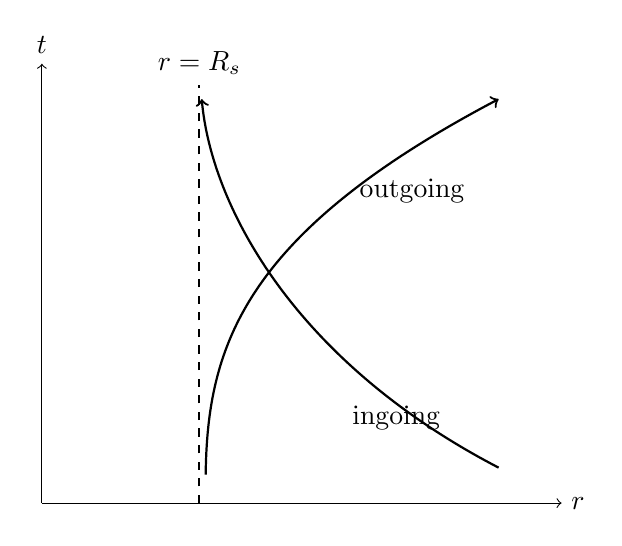
\begin{tikzpicture}[x=1.0cm,y=0.9cm]
\draw[->] (0,0) -- (6.6,0) node[right] {$r$};
\draw[->] (0,0) -- (0,6.2) node[above] {$t$};
\draw[dashed,thick] (2.0,0) -- (2.0,5.9) node[above] {$r=R_s$};
\draw[thick,->] (2.08,.4) .. controls (2.10,2.2) and (2.55,3.8) .. (5.8,5.7);
\draw[thick,->] (5.8,.5) .. controls (3.2,2.0) and (2.15,4.2) .. (2.03,5.7);
\node[align=center] at (4.7,4.4) {outgoing};
\node[align=center] at (4.5,1.2) {ingoing};
\end{tikzpicture}
\caption{A cleaned coordinate-time version of the board sketch.  The apparent slowing is a statement about Schwarzschild \(t\), not about a local failure of light to move at \(c\).}
\end{figure}

Inside the horizon the future light cones tip so far inward that both future-directed radial branches lead toward decreasing \(r\).  No signal originating there can escape to the exterior, and every future-directed causal path reaches the singularity.

\begin{classroomqa}
\audiencequestion{If the speed of light is invariant, what exactly does it mean to say that light slows down near the horizon?\lecturetimestamp{00:31:44}}
\lecturerresponse{The displayed quantity is \(dr/dt\) in a particular coordinate system.  Numerical speed already changes when meters are replaced by centimeters; here the effective radial and temporal calibrations vary with position.  The universal statement is that every light ray follows a null trajectory, \(ds^2=0\).}
\end{classroomqa}
\editorialnote{A freely falling local observer measures vacuum light at \(c\); the vanishing Schwarzschild-coordinate speed at the horizon is not a local observable.}

\begin{classroomqa}
\audiencequestion{Does the same null-speed statement hold regardless of the material medium through which light travels?\lecturetimestamp{00:33:24}}
\lecturerresponse{No.  The available recognition preserves no longer explanation of this answer.}
\end{classroomqa}
\editorialnote{The null-speed claim concerns propagation in vacuum spacetime.  Interactions with matter can give a wave packet a smaller effective speed; that is a property of the medium, not a change in the local causal speed \(c\).}

\begin{classroomqa}
\audiencequestion{What does an incoming light ray look like on the same \(t\)-\(r\) diagram?\lecturetimestamp{00:33:32}}
\lecturerresponse{It is the reverse-looking branch: from large \(r\) it bends toward the horizon and approaches it asymptotically.  It takes an infinite amount of the coordinate time \(t\) to arrive.}
\end{classroomqa}
\editorialnote{An infalling observer reaches and crosses the horizon in finite proper time; only Schwarzschild \(t\) diverges.}

\section{Why Evaporation Creates a Problem}

The horizon deserves much more study: how it forms, what an infalling observer sees, and whether anything locally unusual occurs there.  Susskind defers those questions and jumps to quantum mechanics.  From the outside, matter and all its distinguishing information become squeezed ever closer to the horizon and unavailable.  That alone need not destroy information; it may simply hide it.

Hawking's result makes the issue acute.  A settled classical black hole looks like the dullest object imaginable: spherical, dark, and unable to send a message.  But ``black'' has two meanings.  It can mean emitting nothing, or it can mean emitting thermal black-body radiation.  A quantum black hole is black in the second sense.  It has a temperature, glows, and loses energy.  Since
\begin{equation}
E=Mc^2,
\qquad
R_s=\frac{2GM}{c^2},
\end{equation}
radiation decreases both its mass and its horizon radius.  If evaporation eventually removes the hole, what becomes of the information that appeared to remain at its horizon?  It might be destroyed, trapped in a tiny remnant, or encoded in the outgoing radiation.  The tension among those possibilities is the information problem, and string theory will later help to sharpen its resolution.

No calculation of quantum fields in curved spacetime is attempted tonight.  Instead Susskind follows Bekenstein's simpler route: first understand entropy as information, then calculate how much information a black hole can hide.

\section{Information That Is Present but Hidden}

Imagine dividing a box into cells small enough that each cell is either occupied or empty.  A binary string---one answer per cell---distinguishes the configuration from every other allowed configuration.  More realistic matter requires questions about particle species and other degrees of freedom, but the principle is unchanged: information is measured by the minimum number of yes--no questions required to specify the state.

\begin{classroomqa}
\audiencequestion{Is this only a description of a static system?\lecturetimestamp{00:45:49}}
\lecturerresponse{It is an instantaneous description, at one moment of time.  Dynamics then maps that state to another state.}
\end{classroomqa}

The next principle is deeper: closed-system evolution does not merge two distinct microscopic states into one.  If two configurations differ now, their evolved configurations remain distinguishable in principle.  Classical Hamiltonian evolution is invertible and quantum evolution is unitary.\editorialnote{Dissipative effective equations can erase distinctions only because unobserved environmental degrees of freedom have been omitted; the complete closed state retains them.}

The bathtub makes the difference between loss and inaccessibility concrete.  Two streams of drops could encode two different Morse-code texts.  After the water settles, both tubs look alike.  The visible ripples have gone, yet a complete microscopic measurement would still find different molecular configurations.  The message has spread into degrees of freedom too small and numerous to track.

Entropy is this hidden information.  Relative to the macroscopic questions we can ask---temperature, total energy, composition, water level---many microscopic distinctions remain possible but inaccessible.  In the lecture's bit-counting language,
\begin{equation}
S=\hbox{number of hidden bits}.
\end{equation}
The precise statistical formula is \(S=k_B\ln\Omega\), but the qualitative definition is enough for the black-hole argument.

\section{Temperature as the Cost of Hiding a Bit}

Temperature is familiar to measure and surprisingly indirect to define.  Susskind chooses entropy and energy as the primitive concepts.  Suppose a computer bit is reset to a standard value.  The physical device remains, but the distinction between its former zero and one states disappears from the computer.  It cannot disappear from the complete world; it is transferred to microscopic degrees of freedom in the environment, which heat by a small amount.  This is Landauer's principle.

If one entropy unit is one bit and temperature is measured in energy units, the lecture writes
\begin{align}
\Delta S&=1,\\
\Delta E&=T\,\Delta S,\\
dE&=T\,dS.
\label{eq:first-law}
\end{align}

\begin{figure}[htbp]
\centering

\includegraphics[width=0.84\textwidth]{lecture_02_figure_04.png}
\caption{The board's information-theoretic thermodynamics: \(S\) is entropy, one hidden bit has \(\Delta S=1\), and its minimum energy cost is written \(\Delta E=T\Delta S\).}
\lectureframe{00:58:40.000}
\end{figure}

\editorialnote{In conventional units the reversible erasure cost of one binary bit is \(k_BT\ln2\).  Equation~\eqref{eq:first-law} uses \(k_B=1\) and treats the lecture's entropy unit as one bit while suppressing the associated \(\ln2\).  These conventions do not affect the scaling argument that follows.}

An audience estimate puts the minimum temperature rise from erasing roughly \(100\) gigabytes into a glass of water near \(10^{-15}\) degrees.  Susskind accepts the point rather than the exact number: at room temperature one bit carries an extraordinarily small minimum energy, and real computers dissipate much more because erasure is not performed reversibly.

\begin{classroomqa}
\audiencequestion{Is the hard-drive example only an analogy, or is erasure heating a real law?\lecturetimestamp{01:00:02}}
\lecturerresponse{It is a real physical constraint, Landauer's rule.  Resetting a memory cell removes the old distinction from the computer, so that information must be carried into the environment.  Ordinary operations are far less efficient than the ideal minimum because they also drive circuits, move charges, and create unrelated heat.}
\end{classroomqa}

\begin{classroomqa}
\audiencequestion{Does hiding one bit cost more energy at a higher temperature?\lecturetimestamp{01:02:07}}
\lecturerresponse{Yes.  The relation \(dE=T\,dS\) says exactly that: for the same entropy transfer, a hotter heat bath requires the larger energy transfer.  One may equally regard this energy-per-hidden-bit relation as the definition of temperature.}
\end{classroomqa}

\begin{classroomqa}
\audiencequestion{If one writes over a previously stored bit, has that old information been lost?\lecturetimestamp{01:02:43}}
\lecturerresponse{It has left the computer, but it has not vanished from the closed physical system.  The overwritten distinction has been dispersed into the environment, where it contributes inaccessible information and therefore entropy.}
\end{classroomqa}

The identification of thermodynamic entropy with missing microscopic information goes back to Boltzmann; Shannon gave the corresponding information-theoretic language in the twentieth century.  Susskind remarks that this explanation was strangely absent from the thermodynamics courses he and members of the audience encountered in the 1950s.  Computer science made the connection harder to overlook, but did not originate its physical content.

\section{Putting One Bit into a Black Hole}

We can now build a black hole conceptually, bit by bit, just as a bathtub can be filled drop by drop.  The question is differential: when one additional bit is hidden, how much does the horizon grow?  Begin with a hole of mass \(M\) and radius \(R_s\), then send in the simplest object whose only recoverable distinction is whether it was absorbed.

\begin{classroomqa}
\audiencequestion{Doesn't the information require infinite coordinate time to enter the hole?\lecturetimestamp{01:08:07}}
\lecturerresponse{It becomes exponentially compressed near the horizon and unavailable to the exterior in a short practical time, even though Schwarzschild coordinate time assigns the actual crossing an infinite value.  For the outside accounting it can therefore be treated as stored at the horizon.}
\end{classroomqa}

A photon is a natural candidate, but a generic photon carries more than one bit.  Its polarization may encode a binary choice.  A sharply localized arrival point supplies many further yes--no questions: upper or lower hemisphere, left or right half, and so on.  Quantum mechanics limits localization to roughly a wavelength, so the way to suppress positional information is to use the longest wavelength the hole can still absorb.

\begin{classroomqa}
\audiencequestion{Is there really an upper wavelength beyond which the photon cannot enter?\lecturetimestamp{01:12:15}}
\lecturerresponse{Yes.  A wave much larger than the hole is predominantly scattered rather than absorbed.  The useful marginal choice is a wavelength comparable to the horizon radius: long enough to wash out the point of entry, yet short enough to have a substantial absorption probability.}
\end{classroomqa}

\begin{classroomqa}
\audiencequestion{Does the direction from which the photon arrives itself add information?\lecturetimestamp{01:13:28}}
\lecturerresponse{For a wavelength of order the whole horizon, the field varies so slowly across the hole that the arrival direction cannot be resolved with fine precision.  This is why the long-wavelength limit approximates a single yes--no datum rather than a sharply located impact.}
\end{classroomqa}

Thus choose, at order of magnitude,
\begin{equation}
\lambda\sim R_s=\frac{2GM}{c^2}.
\label{eq:one-bit-wave}
\end{equation}
Photon kinematics gives
\begin{equation}
E=cp,
\qquad
p=\hbar k=\frac{h}{\lambda},
\qquad
\Delta E\sim\frac{\hbar c}{R_s}.
\label{eq:one-bit-energy}
\end{equation}
Here \(k=2\pi/\lambda\) and \(h=2\pi\hbar\).  The lecture deliberately ignores the \(2\pi\), as well as order-one absorption factors.

\begin{classroomqa}
\audiencequestion{Should momentum be written \(\hbar/\lambda\), or \(h/\lambda\)?\lecturetimestamp{01:16:00}}
\lecturerresponse{With \(\lambda\) the ordinary wavelength, the exact relation is \(p=h/\lambda=2\pi\hbar/\lambda\); with wave number \(k=2\pi/\lambda\), it is \(p=\hbar k\).  The present estimate keeps only the scale, so the factor \(2\pi\) is intentionally discarded.}
\end{classroomqa}

The energy cost of hiding one bit is the temperature scale.  Equations~\eqref{eq:one-bit-wave} and~\eqref{eq:one-bit-energy} therefore give
\begin{equation}
k_BT_H\sim\frac{\hbar c}{R_s}
\sim\frac{\hbar c^3}{GM}.
\end{equation}
The exact Hawking result is
\begin{equation}
k_BT_H=\frac{\hbar c^3}{8\pi GM}.
\end{equation}
The elementary argument gets the dependence on \(M,G,c,\hbar\), but not the coefficient.

\section{One Bit Occupies One Planck-Scale Patch}

The same photon tells us how the horizon grows.  Its energy changes the mass by
\begin{equation}
\Delta M=\frac{\Delta E}{c^2}
\sim\frac{\hbar}{cR_s}.
\end{equation}
Since \(R_s=2GM/c^2\),
\begin{equation}
\Delta R_s=\frac{2G}{c^2}\Delta M
\sim\frac{G\hbar}{c^3R_s},
\end{equation}
where all order-one factors have again been suppressed.  Multiplying by \(R_s\),
\begin{equation}
R_s\Delta R_s\sim\frac{G\hbar}{c^3}.
\end{equation}
Because \(A=4\pi R_s^2\), its differential is \(dA=8\pi R_s\,dR_s\).  Therefore
\begin{equation}
\Delta A\sim\frac{G\hbar}{c^3}=\ell_P^2,
\qquad
\ell_P=\sqrt{\frac{G\hbar}{c^3}}.
\label{eq:planck-patch}
\end{equation}

\begin{figure}[htbp]
\centering

\includegraphics[width=0.84\textwidth]{lecture_02_figure_05.png}
\caption{The completed scaling argument on the board: the one-bit energy \(\Delta E\sim\hbar c/R_s\) leads to a radius-squared, hence area, increment of order \(G\hbar/c^3\).}
\lectureframe{01:22:40.000}
\end{figure}

During the live calculation, factors of \(c\) are restored halfway through and an audience member catches the missing \(c^{-2}\) in the Schwarzschild radius.  That correction is exactly what produces the \(c^{-3}\) in Equation~\eqref{eq:planck-patch}.

\begin{classroomqa}
\audiencequestion{Did restoring \(c\) in only part of the calculation lose two powers of it?\lecturetimestamp{01:21:18}}
\lecturerresponse{Yes.  The dimensional relation is \(R_s=2GM/c^2\), not simply \(2GM\).  Restoring that factor makes the area scale \(G\hbar/c^3\).}
\end{classroomqa}

Using \(G\simeq6.7\times10^{-11}\,\mathrm{m^3\,kg^{-1}\,s^{-2}}\), \(\hbar\simeq1.05\times10^{-34}\,\mathrm{J\,s}\), and \(c^3\simeq2.7\times10^{25}\,\mathrm{m^3\,s^{-3}}\),
\begin{equation}
\ell_P^2\simeq2.6\times10^{-70}\,\mathrm{m^2},
\qquad
\ell_P\simeq1.6\times10^{-35}\,\mathrm{m}.
\end{equation}
The lecture's spoken powers wander while the estimate is done at the board; the physical conclusion is stable.  This scale is far below direct experimental resolution.

The memorable image is of impenetrable bits with sharp elbows, accumulating on the horizon and pushing one another aside.  Each new bit claims approximately one Planck-area patch.  It is a metaphor for the area accounting, not a claim that literal square tiles form the horizon.

\begin{classroomqa}
\audiencequestion{If the first photon is still approaching when another photon enlarges the horizon, doesn't the old one become located inside the new horizon?\lecturetimestamp{01:26:39}}
\lecturerresponse{The simple static picture is not precise enough to settle that question.  The event horizon in a dynamical spacetime must be defined globally, and its location changes as matter arrives.  In the exterior description used here, the information remains associated with the growing horizon.  A careful definition of that horizon is deferred.}
\end{classroomqa}

\begin{classroomqa}
\audiencequestion{Would the same issue arise when a huge mass is added, for example when two black holes collide?\lecturetimestamp{01:27:03}}
\lecturerresponse{Yes; then the dynamical character is impossible to ignore.  The lecture postpones the full merger geometry until the horizon has been defined more carefully.}
\end{classroomqa}

\begin{classroomqa}
\audiencequestion{Is a Planck area defined only on a flat patch, rather than on a spherical horizon?\lecturetimestamp{01:27:30}}
\lecturerresponse{It is an area scale on the spherical surface, not a requirement that the horizon be flat.  The planar-versus-spherical distinction is not significant for this counting.}
\end{classroomqa}
\editorialnote{When the horizon curvature radius is enormous compared with \(\ell_P\), each Planck-size neighborhood is locally almost flat.}

For a hole eight kilometers across, the marginal photon is correspondingly a long radio wave of roughly that scale.  An audience analogy compares the size-independent area increment with adding the same extra circumference to a string wrapped around a basketball or around Earth: in each case the radial gap created by a fixed added circumference is the same.  The exact geometries differ, but both examples isolate a change that is independent of the object's original size.

\section{The Area Law}

Adding one bit at a time changes the horizon area by a universal microscopic amount.  The number of bits that can be hidden must therefore be proportional to \(A/\ell_P^2\), not to the volume.  Bekenstein inferred the proportionality; Hawking's calculation fixed its coefficient:
\begin{equation}
S_{\mathrm{BH}}=\frac{k_B A c^3}{4G\hbar}
=\frac{k_B A}{4\ell_P^2}.
\label{eq:bh-entropy}
\end{equation}
If entropy is counted in binary bits rather than thermodynamic units, divide \(S_{\mathrm{BH}}/k_B\) by \(\ln2\).

\begin{figure}[htbp]
\centering

\includegraphics[width=0.84\textwidth]{lecture_02_figure_06.png}
\caption{The final board formula, including Hawking's factor \(1/4\): \(S\propto Ac^3/(4G\hbar)\) in the lecture's entropy units.}
\lectureframe{01:31:02.000}
\end{figure}

Black holes therefore have more entropy than ordinary systems of comparable size, by an enormous margin.  Yet the answer is still smaller than a naive volume count might suggest.  The independent information is bounded by a surface measure.  This inversion---a three-dimensional gravitating region described by information scaling as a two-dimensional boundary---is the seed of the holographic principle.

\begin{classroomqa}
\audiencequestion{Where does the factor \(1/4\) in the entropy formula come from?\lecturetimestamp{01:30:30}}
\lecturerresponse{Bekenstein's argument fixed the dependence on area and the fundamental constants but left an unknown coefficient; his estimates produced possibilities such as logarithms of two.  Hawking's quantum-field calculation fixed the coefficient to precisely \(1/4\).}
\end{classroomqa}

The position of \(\hbar\) contains the final surprise.  One might expect a quantum entropy to be proportional to \(\hbar\) and vanish in the classical limit.  Instead \(\hbar\) is in the denominator.  As \(\hbar\to0\), a wave can carry arbitrarily fine information at arbitrarily small energy cost, so the entropy capacity diverges.  Quantization does not add a tiny entropy to an otherwise classical hole; it prevents the information capacity from being infinite.

\begin{classroomqa}
\audiencequestion{Why does \(\hbar\), whose units are angular momentum, also set the relation between ordinary momentum and wavelength?\lecturetimestamp{01:33:23}}
\lecturerresponse{\(\hbar\) has units of action, equivalently momentum times distance.  Since \(p\lambda\) has those same units, the quantum relation can be \(p\sim\hbar/\lambda\) up to the \(2\pi\) convention.  Angular momentum \(\mathbf r\times\mathbf p\) carries the same dimensions for the same reason.}
\end{classroomqa}

The lecture stops here, not because the subject is exhausted but because this is the right boundary.  Geometry has told us why the horizon hides information; thermodynamics has told us how to count hidden information; quantum mechanics has supplied a finite area per bit.  The next question is no longer whether a black hole has microscopic states, but how those states encode and eventually return what fell in.
